% ------------------------------------------------- %
% ---------------------- MOTIVATION ---------------- %
% ------------------------------------------------- %
\section{Motivation}

Modern official statistics operate under a fundamental constraint: survey data ($S$, containing $\mathbf{x}_i, y_i$) is characterized by a high signal-to-noise ratio but is expensive to collect and essentially sparse. Conversely, administrative or historical data (Frame $U$, containing $\mathbf{z}_i$) is ubiquitous and inexpensive but often suffers from data drift, concept drift, or definitional mismatches relative to the current study target.

Our goal is not merely to impute missing data arising from item non-response. Rather, we aim to leverage the ``cheap'' frame data ($\mathbf{z}_i$) to reduce the variance of estimates derived from the ``expensive'' sample data ($\mathbf{x}_i$), while maintaining robustness against model failure.

It is important to clarify the scope of this work. We do not propose a novel class of estimators. Instead, our objective is to benchmark how existing theoretical frameworks—specifically Model-Calibration and Doubly Robust estimation—perform when applied to the specific constraint of fusing dense historical records with missing current survey data. We analyze this in the context of \textit{Prediction-Powered Inference} (PPI), adapting machine learning tools to finite population survey inference.

\begin{figure}[H]
  \centering
  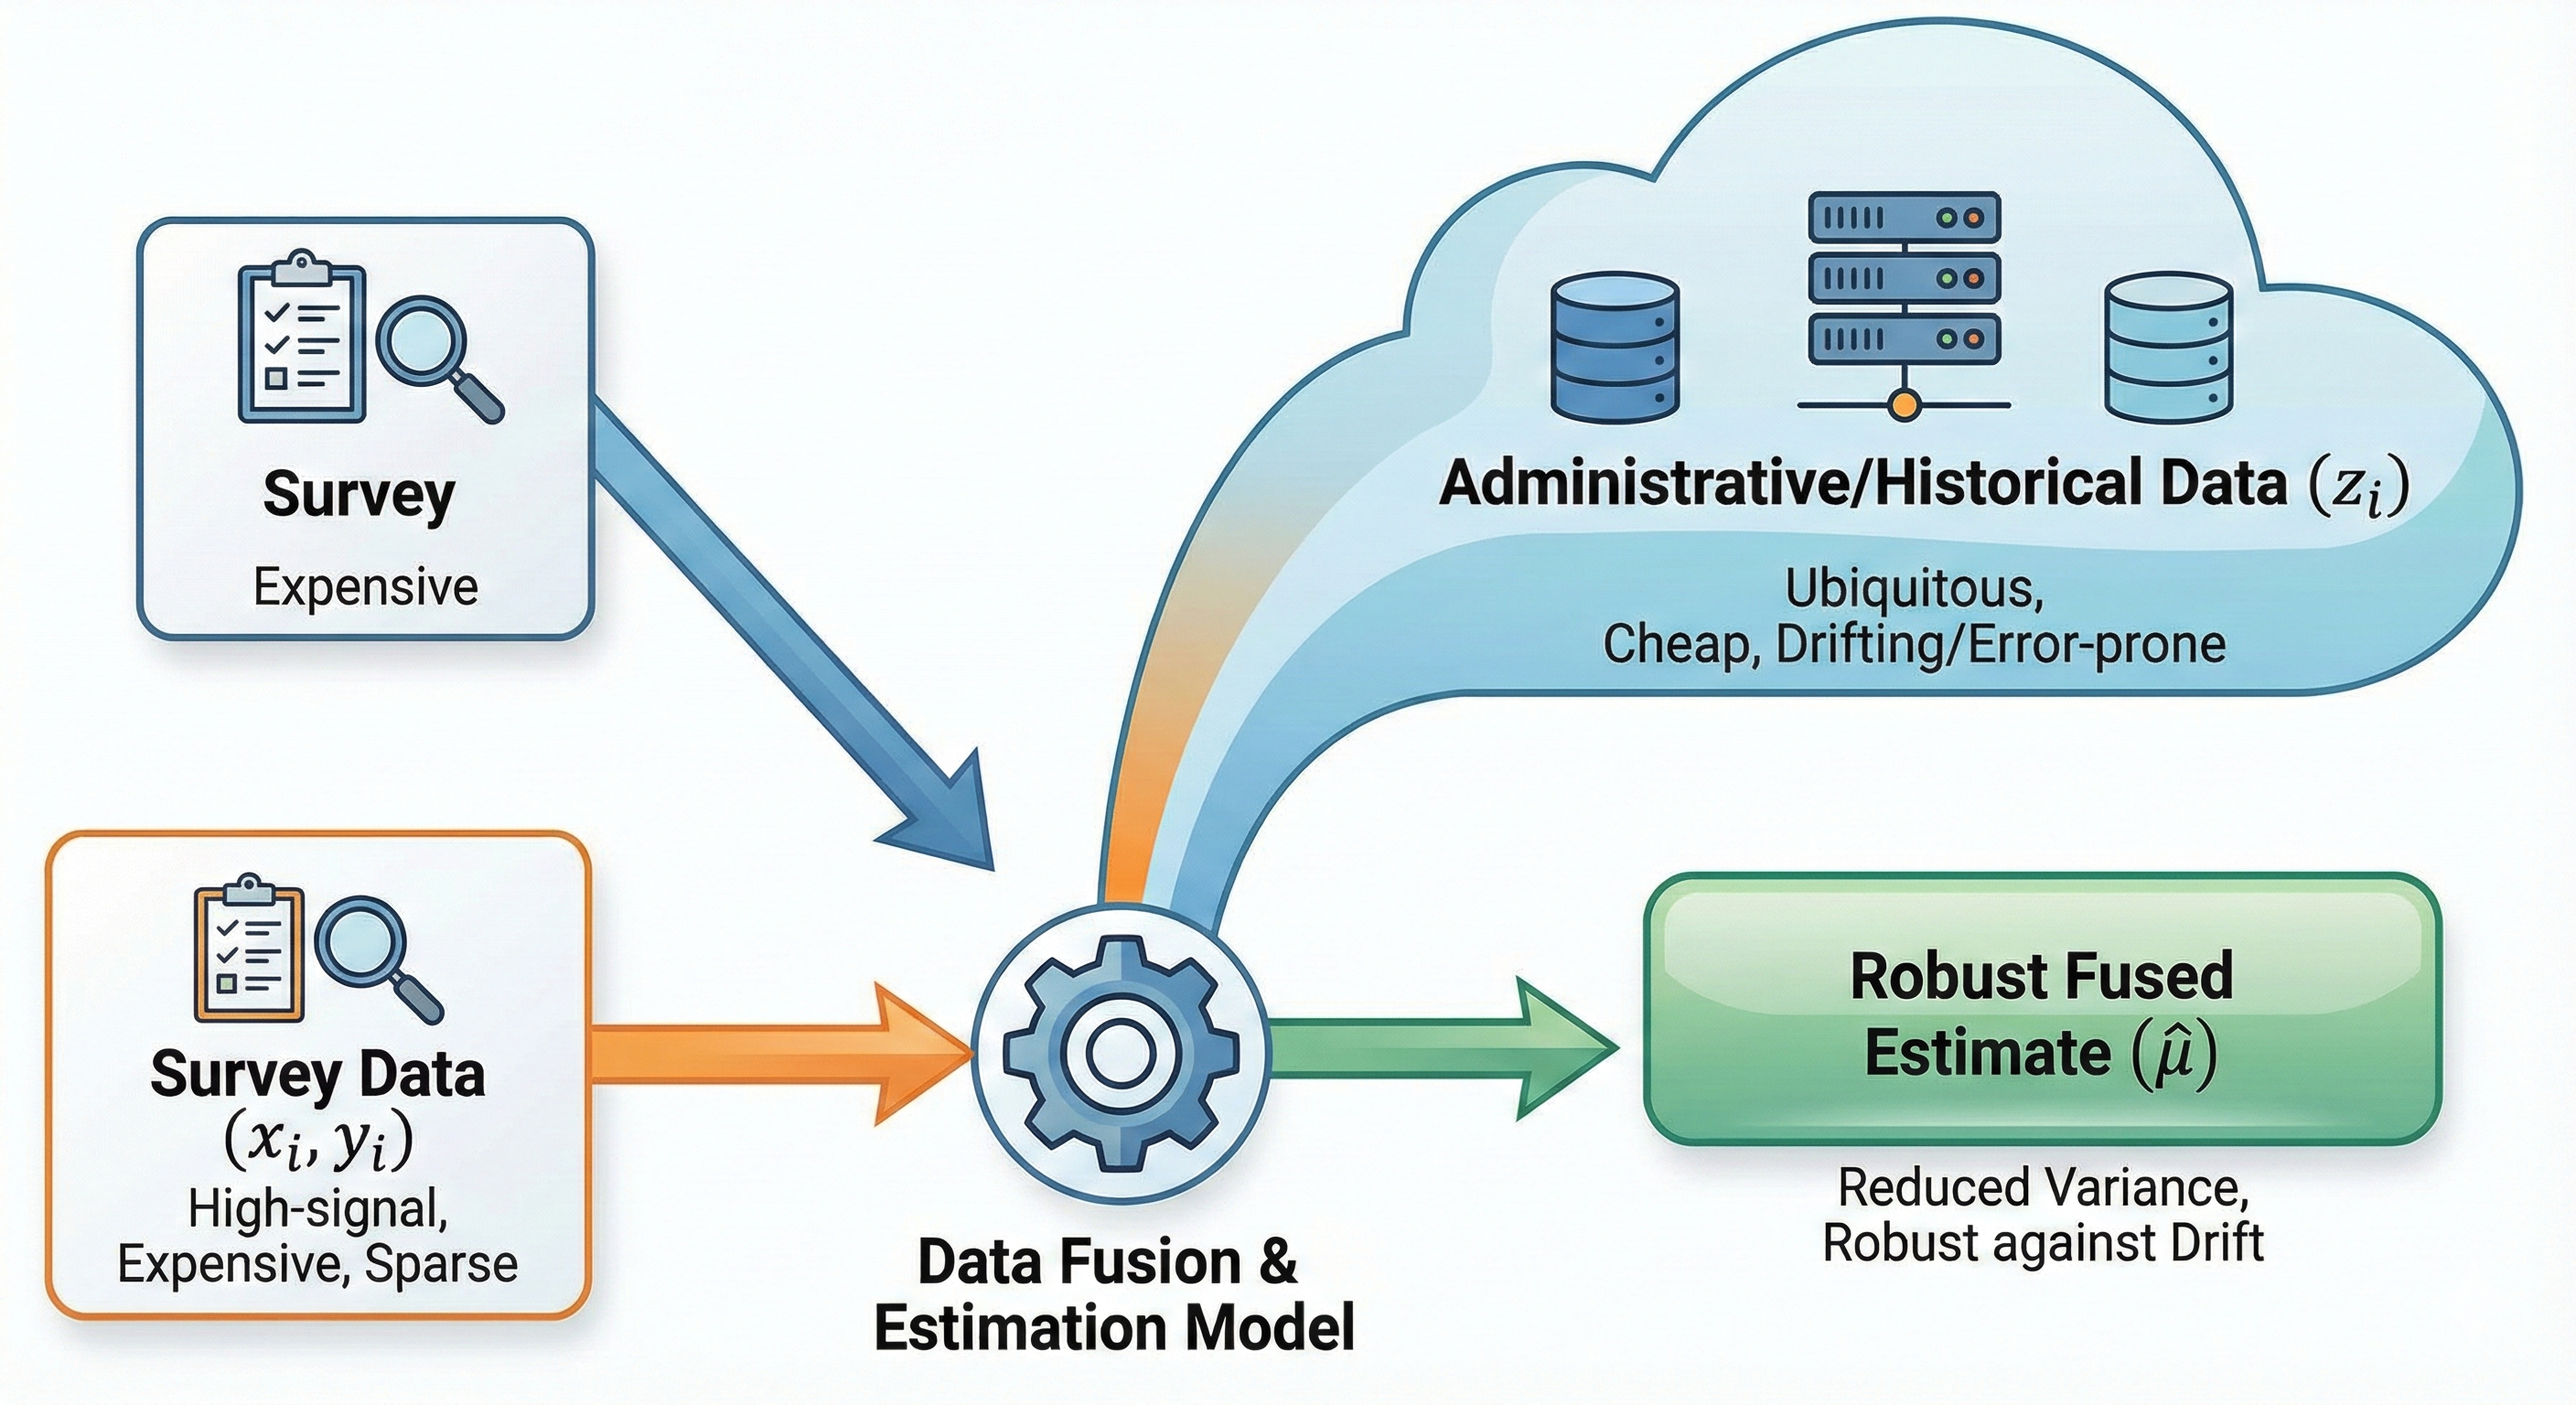
\includegraphics[width=0.8\textwidth]{paper/diagrams/1A.png}
\end{figure}

% ------------------------------------------------- %
% ------------ SCENARIOS OF MISSING DATA ---------- %
% ------------------------------------------------- %
\section{Scenarios of Missing Data}
We define the population, sampling design, and missing data mechanisms as follows:

\begin{description}
    \item[Population ($U$):] A finite population of size $N$, denoted $U=\{1,2,\dots,N\}$.
    
    \item[Sample ($S$):] A probability sample of size $n$ drawn from $U$, such that $S\subseteq U$ and $|S|=n$.
    
    \item[Inclusion probabilities and weights:] Let $\pi_i=\Pr(i\in S)>0$ be the first-order inclusion probability. The design weights are defined as $d_i := 1/\pi_i$ for $i\in S$. (We assume $\pi_{ij}=\Pr(i,j\in S) >0$ for variance estimation where required).
    
    \item[Frame auxiliaries:] A vector $\mathbf{z}_i\in\mathbb{R}^{p_z}$ available for \emph{every} unit $i\in U$ (e.g., census or administrative data).
    
    \item[Sample auxiliaries:] A vector $\mathbf{x}_i\in\mathbb{R}^{p_x}$ observed for \emph{all} units $i\in S$.
    
    \item[Imputation vector:] We define the generic predictor vector $\mathbf{v}_i \in \mathbb{R}^{p_v}$ used for imputation models. 
    \[
    \mathbf{v}_i := \begin{cases} 
      \mathbf{x}_i & \text{in Scenario 1 (Standard Survey Setting)} \\
      [\mathbf{z}_i, \mathbf{x}_i]^\top & \text{in Scenarios using Frame Data}
   \end{cases}
    \]
    
    \item[Study variable and Item Indicator:] Let $y_i\in\mathbb{R}$ be the variable of interest. For each $i\in S$, define the \emph{item-response} indicator $r_i=\mathbbm{1}\{y_i\ \text{is observed}\}\in\{0,1\}$. We observe $y_i$ if and only if  $r_i = 1$.
    
    \item[Unit Response:] Let $R_i \in \{0,1\}$ denote the indicator that a sampled unit $i \in S$ participates in the survey (providing at least the auxiliary vector $\mathbf{x}_i$). We assume full unit response, such that $R_i = 1$ for all $i \in S$. Consequently, any missingness is restricted solely to item nonresponse in $y_i$ (captured by $r_i$).
    
    \item[Historical Data:] Let $t$ denote the current time period. Variables without temporal superscripts refer to the current period ($y_i, \mathbf{x}_i, \mathbf{z}_i$). Historical data from $k$ periods prior are denoted $y_i^{(t-k)}, \mathbf{x}_i^{(t-k)}, \mathbf{z}_i^{(t-k)}$. In our primary application, we have complete census data (or rich historical surveys) from period $t-1$ (or up to $t-1$) and a smaller survey sample from the current period $t$.
    
    \item[Missing at Random (MAR):] We assume the missing data mechanism for $y_i$ is Missing at Random given the predictors $\mathbf{v}_i$. Since $R_i \equiv 1$:
    \[
    \Pr(r_i=1 \mid y_i,\mathbf{v}_i) \;=\; \Pr(r_i=1 \mid \mathbf{v}_i).
    \]
    We denote the response propensity as $\rho_i(\mathbf{v}_i) := \Pr(r_i=1\mid \mathbf{v}_i)$.
    
    \item[Sets and counts:] We partition the sample $S$ into respondents $S_r$ and non-respondents $S_m$:
    \[ 
    S_r = \{ i \in S : r_i = 1\}, \qquad S_m = \{ i \in S : r_i = 0\}, \qquad n_r = |S_r|. 
    \]
\end{description}

\noindent\textbf{Observed-data summary:} For each unit $i\in S$, we observe the tuple:
\[ 
(\, \mathbf{x}_i,\ \mathbf{z}_i,\ d_i,\ r_i,\ y_i^{\mathrm{obs}}\,) 
\]

Imputation of missing $y_i$ relies on models fit within $S$ using available predictors. In contrast, projection estimators (discussed later) utilize predictions $f(\mathbf{z}_i)$ available for all $i \in U$, where $f$ is a model pre-trained on historical data or data external to the current sample $S$.

\paragraph{Baseline (Complete Response, Current Period Only).} 
If $y_i$ were observed for all $i \in S$, the unbiased Horvitz-Thompson estimator for the population mean $\bar{Y}$ is:
\begin{equation} \label{eq:baseline_ht}
\hat{\mu}_{\mathrm{HT}} = \frac{1}{N} \sum_{i \in S} d_i\, y_i, \qquad d_i := \frac{1}{\pi_i}.
\end{equation}

% ------------------------------------------------- %
% ------------------ SCENARIO 1 ------------------- %
% ------------------------------------------------- %
\paragraph{Scenario 1: Item Nonresponse.}
We first consider the scenario where the response variable $y_i$ is subject to missingness. Standard approaches in survey literature to handle nonresponse generally fall into three categories: Imputation, Re-weighting, and Doubly Robust methods.

Recall that $S_r = \{i \in S: r_i=1\}$ denotes the set of respondents, and $S_m = \{i \in S: r_i=0\}$ the set of missing units. In this scenario, we assume predictors $\mathbf{x}_i$ are available for all $i \in S$, but we do not yet utilize external frame data.


\medskip
\noindent \textbf{1. Imputation Estimator} \parencite[e.g.,]{kalton_kasprzyk_1986_surveymeth,dagdoug_goga_haziza_2025_sjs}:
This approach predicts missing values using a model fit on the responding units.
\begin{equation} \label{eq:s1_imp}
\hat{\mu}_{\text{imp}} = \frac{1}{N}\left(\sum_{i\in S_r}\frac{y_i}{\pi_i} + \sum_{i\in S_m}\frac{\hat{m}_{S_{r}}(\mathbf{x}_i)}{\pi_i}\right) 
\end{equation}
where $\hat{m}_{S_{r}}(\mathbf{x}_i)$ is the predicted value for unit $i$ obtained from a model trained on $(y_i, \mathbf{x}_i)$ for $i \in S_r$.

\medskip
\noindent \textbf{2. Nonresponse Weighting Adjusted (NWA) Estimator} \parencite{oh_scheuren_1983_incomplete,fay_1991_design_based,little_rubin_2002_samd}:
Often referred to as the Inverse Probability Weighting (IPW) estimator, this approach adjusts the sampling weights by the estimated response probability, $\hat{p}_i = \widehat{\Pr}(r_i=1 \mid \mathbf{x}_i)$.
\begin{equation} \label{eq:s1_nwa}
\hat{\mu}_{\text{NWA}} = \frac{1}{N}\sum_{i\in S_r}\frac{y_i}{\pi_i \hat{p}_i} 
\end{equation}

\medskip
\noindent \textbf{3. Doubly Robust (AIPW) Estimator} \parencite{robins_rotnitzky_zhao_1994_jasa,kim_haziza_2014_sinica,Haziza2017}:
This estimator integrates the previous two. It utilizes the imputation model to predict outcomes for the full sample and employs propensity weights to correct the residuals (the difference between observed and predicted values) for the respondents.
\begin{equation} \label{eq:s1_dr}
\hat{\mu}_{\text{DR}} = \frac{1}{N} \sum_{i \in S} \frac{1}{\pi_i} \left[ \hat{m}_{S_{r}}(\mathbf{x}_i) + \frac{r_i}{\hat{p}_i} \left( y_i - \hat{m}_{S_{r}}(\mathbf{x}_i) \right) \right] 
\end{equation}
This estimator is consistent if \textit{either} the imputation model $\hat{m}_{S_{r}}(\cdot)$ \textit{or} the response probability model $\hat{p}_i$ is correctly specified.

% ------------------------------------------------- %
% ------------------ SCENARIO 2 ------------------- %
% ------------------------------------------------- %
\paragraph{Scenario 2: Item Nonresponse with Population Auxiliary Data.}

We now extend the setting to assume access to a vector of auxiliary variables $\mathbf{z}_i$ for every unit in the population $U$ (e.g., census data), in addition to sample-specific information $\mathbf{x}_i$. 

This distinction is critical: $\mathbf{z}_i$ allows for population-level projection, while $\mathbf{x}_i$ is often richer (more predictive) but observed only in the sample. A standard estimator in this setting is the Nonresponse Generalized Regression (NR-GREG) estimator \parencite{sarndal_lundstrom_2005_nonresponse,kott_2006_surveymethodology,kim_park_2010_isr}. This estimator combines a population projection based on $\mathbf{z}_i$ with a bias correction term based on the respondents.

\begin{equation} \label{eq:s2_greg}
\hat{\mu}_{\text{NR-GREG}}
  = \frac{1}{N}\left(
      \sum_{i\in U} \hat{m}_{S_{r}}(\mathbf{z}_i)
      + \sum_{i\in S}
          \frac{r_i}{\hat{p}_i \pi_i} (y_i - \hat{m}_{S_{r}}(\mathbf{z}_i))
    \right),
\end{equation}

\noindent where:
\begin{itemize}
  \item $\hat{m}_{S_r}(\mathbf{z}_i)$ is the predicted value from an outcome model $g(\mathbf{z}_i; \hat{\beta}_{S_r})$ fit on the respondents $S_r$ using \emph{only} the frame auxiliaries $\mathbf{z}_i$. The projection term $\sum_{i\in U} \hat{m}_{S_r}(\mathbf{z}_i)$ therefore depends only on variables available for the entire population.
  
  \item $\hat{p}_i$ is the estimated response probability typically obtained from a model of $r_i$ on the full sample auxiliaries $\mathbf{v}_i = [\mathbf{z}_i,\mathbf{x}_i]$.
\end{itemize}


\medskip
\noindent\textbf{Theoretical Properties:}
This estimator is a specific instance of the calibration estimator and relies on the ``Difference Estimator'' principle \parencite{cassel_sarndal_wretman_1976_biometrika}. The intuition is twofold:
\begin{enumerate}
    \item \textbf{Variance Reduction:} If the model $\hat{m}_{S_{r}}(\mathbf{z}_i)$ is close to the true $y_i$, the variance is greatly reduced.
    \item \textbf{Bias Correction:} The second term acts as a correction based on the residuals $(y_i - \hat{m}_{S_{r}}(\mathbf{z}_i))$ observed among respondents. Even if the outcome model is biased, as long as the propensity weights $\hat{p}_i$ are correctly specified, this term corrects the bias, preserving the \textit{double robustness} property \parencite{kang_schafer_2007_statsci}.
\end{enumerate}

\medskip
\noindent\textbf{Limitation and Motivation:}
A critical limitation of the standard NR-GREG estimator is the restriction on the outcome model. To compute the population projection term $\sum_{i \in U} \hat{m}_{S_{r}}(\cdot)$, the model must depend \textit{only} on variables available for the entire population ($\mathbf{z}_i$). 

Consequently, the richer sample-only auxiliaries $\mathbf{x}_i$ do not enter the outcome model directly; they can only affect the estimate indirectly through the response propensity model $\hat{p}_i(\mathbf{v}_i)$. The predictive power of $\mathbf{x}_i$ is thus lost for the population projection. This motivates the need to strictly distinguish between our data sources:
\begin{itemize}
    \item $\mathbf{x}_i$: Rich auxiliary information available only on the sample $S$ (e.g., detailed clinical measurements).
    \item $\mathbf{z}_i$: Auxiliary information available on the entire frame $U$ (e.g., demographics in administrative records).
\end{itemize}

The next scenario addresses how to integrate these two data sources effectively to leverage the predictive power of $\mathbf{x}_i$ for population inference.

% ------------------------------------------------- %
% ------------------ SCENARIO 3 ------------------- %
% ------------------------------------------------- %
\paragraph{Scenario 3: Two-Step Estimation (Mass Imputation with Projection).}

A critical limitation of the standard NR-GREG (Scenario 2) is that the population projection term must rely strictly on frame variables $\mathbf{z}_i$. In practice, the sample often contains rich variables $\mathbf{x}_i$ that are highly predictive of $y_i$ but missing from the frame. Standard GREG cannot leverage these $\mathbf{x}_i$ variables to adjust the population anchor.

To bridge this gap, we employ a two-step approach, referred to in the literature as the \textbf{Projection Estimator} \parencite{kim_rao_2012_biometrika}, \textbf{Mass Imputation} \parencite{breidt_opsomer_2017_statsci}, or \textbf{Model-Calibration} \parencite{wu_sitter_2001_jasa}. This approach effectively decouples the imputation step (aimed at bias reduction) from the projection step (aimed at variance reduction):

\begin{enumerate}
    \item \textbf{Step 1 (Rich Imputation):} 
    We fit a high-dimensional model $\hat{m}_{\text{imp}}(\mathbf{v}_i)$ on the respondents $S_r$ using the full predictor vector $\mathbf{v}_i = [\mathbf{z}_i, \mathbf{x}_i]$. We then generate predictions $\tilde{y}_i$ for the non-respondents and define the \textit{completed variable} $y_i^\star$ for the entire sample $S$:
    \[ 
    y_i^\star = r_i y_i + (1-r_i)\tilde{y}_i 
    \]
    This step effectively ``mass imputes'' the missing data, reducing nonresponse bias by leveraging the rich sample auxiliaries $\mathbf{x}_i$.
    
    \item \textbf{Step 2 (Frame Projection):} 
    We treat the completed values $y_i^\star$ as the variable of interest. We fit a second, coarser model $\hat{m}_{\text{proj}}(\mathbf{z}_i)$ (often a linear projection or a tree-based model) that relates the completed $y_i^\star$ to the frame variables $\mathbf{z}_i$ available for the whole population.
\end{enumerate}

The resulting estimator is given by:
\begin{equation} \label{eq:s3_mass_imp}
\hat{\mu}_{\text{2step}} = \frac{1}{N} \left( \sum_{i \in U} \hat{m}_{\text{proj}}(\mathbf{z}_i) + \sum_{i \in S} \frac{y_i^\star - \hat{m}_{\text{proj}}(\mathbf{z}_i)}{\pi_i} \right) 
\end{equation}

This estimator combines the advantages of both data sources ("Best of Both Worlds"):
\begin{itemize}
    \item The first term, $\sum_{U} \hat{m}_{\text{proj}}(\mathbf{z}_i)$, leverages the ubiquity of the frame data $\mathbf{z}$ to reduce sampling variance.
    \item The second term acts as a bias correction for the projection model, ensuring consistency.
\end{itemize}

Crucially, because $y_i^\star$ embodies the information contained in $\mathbf{x}_i$ (via Step 1), this method effectively ``imports'' the predictive power of $\mathbf{x}$ into the population estimate without requiring $\mathbf{x}$ to be observed for the entire population.


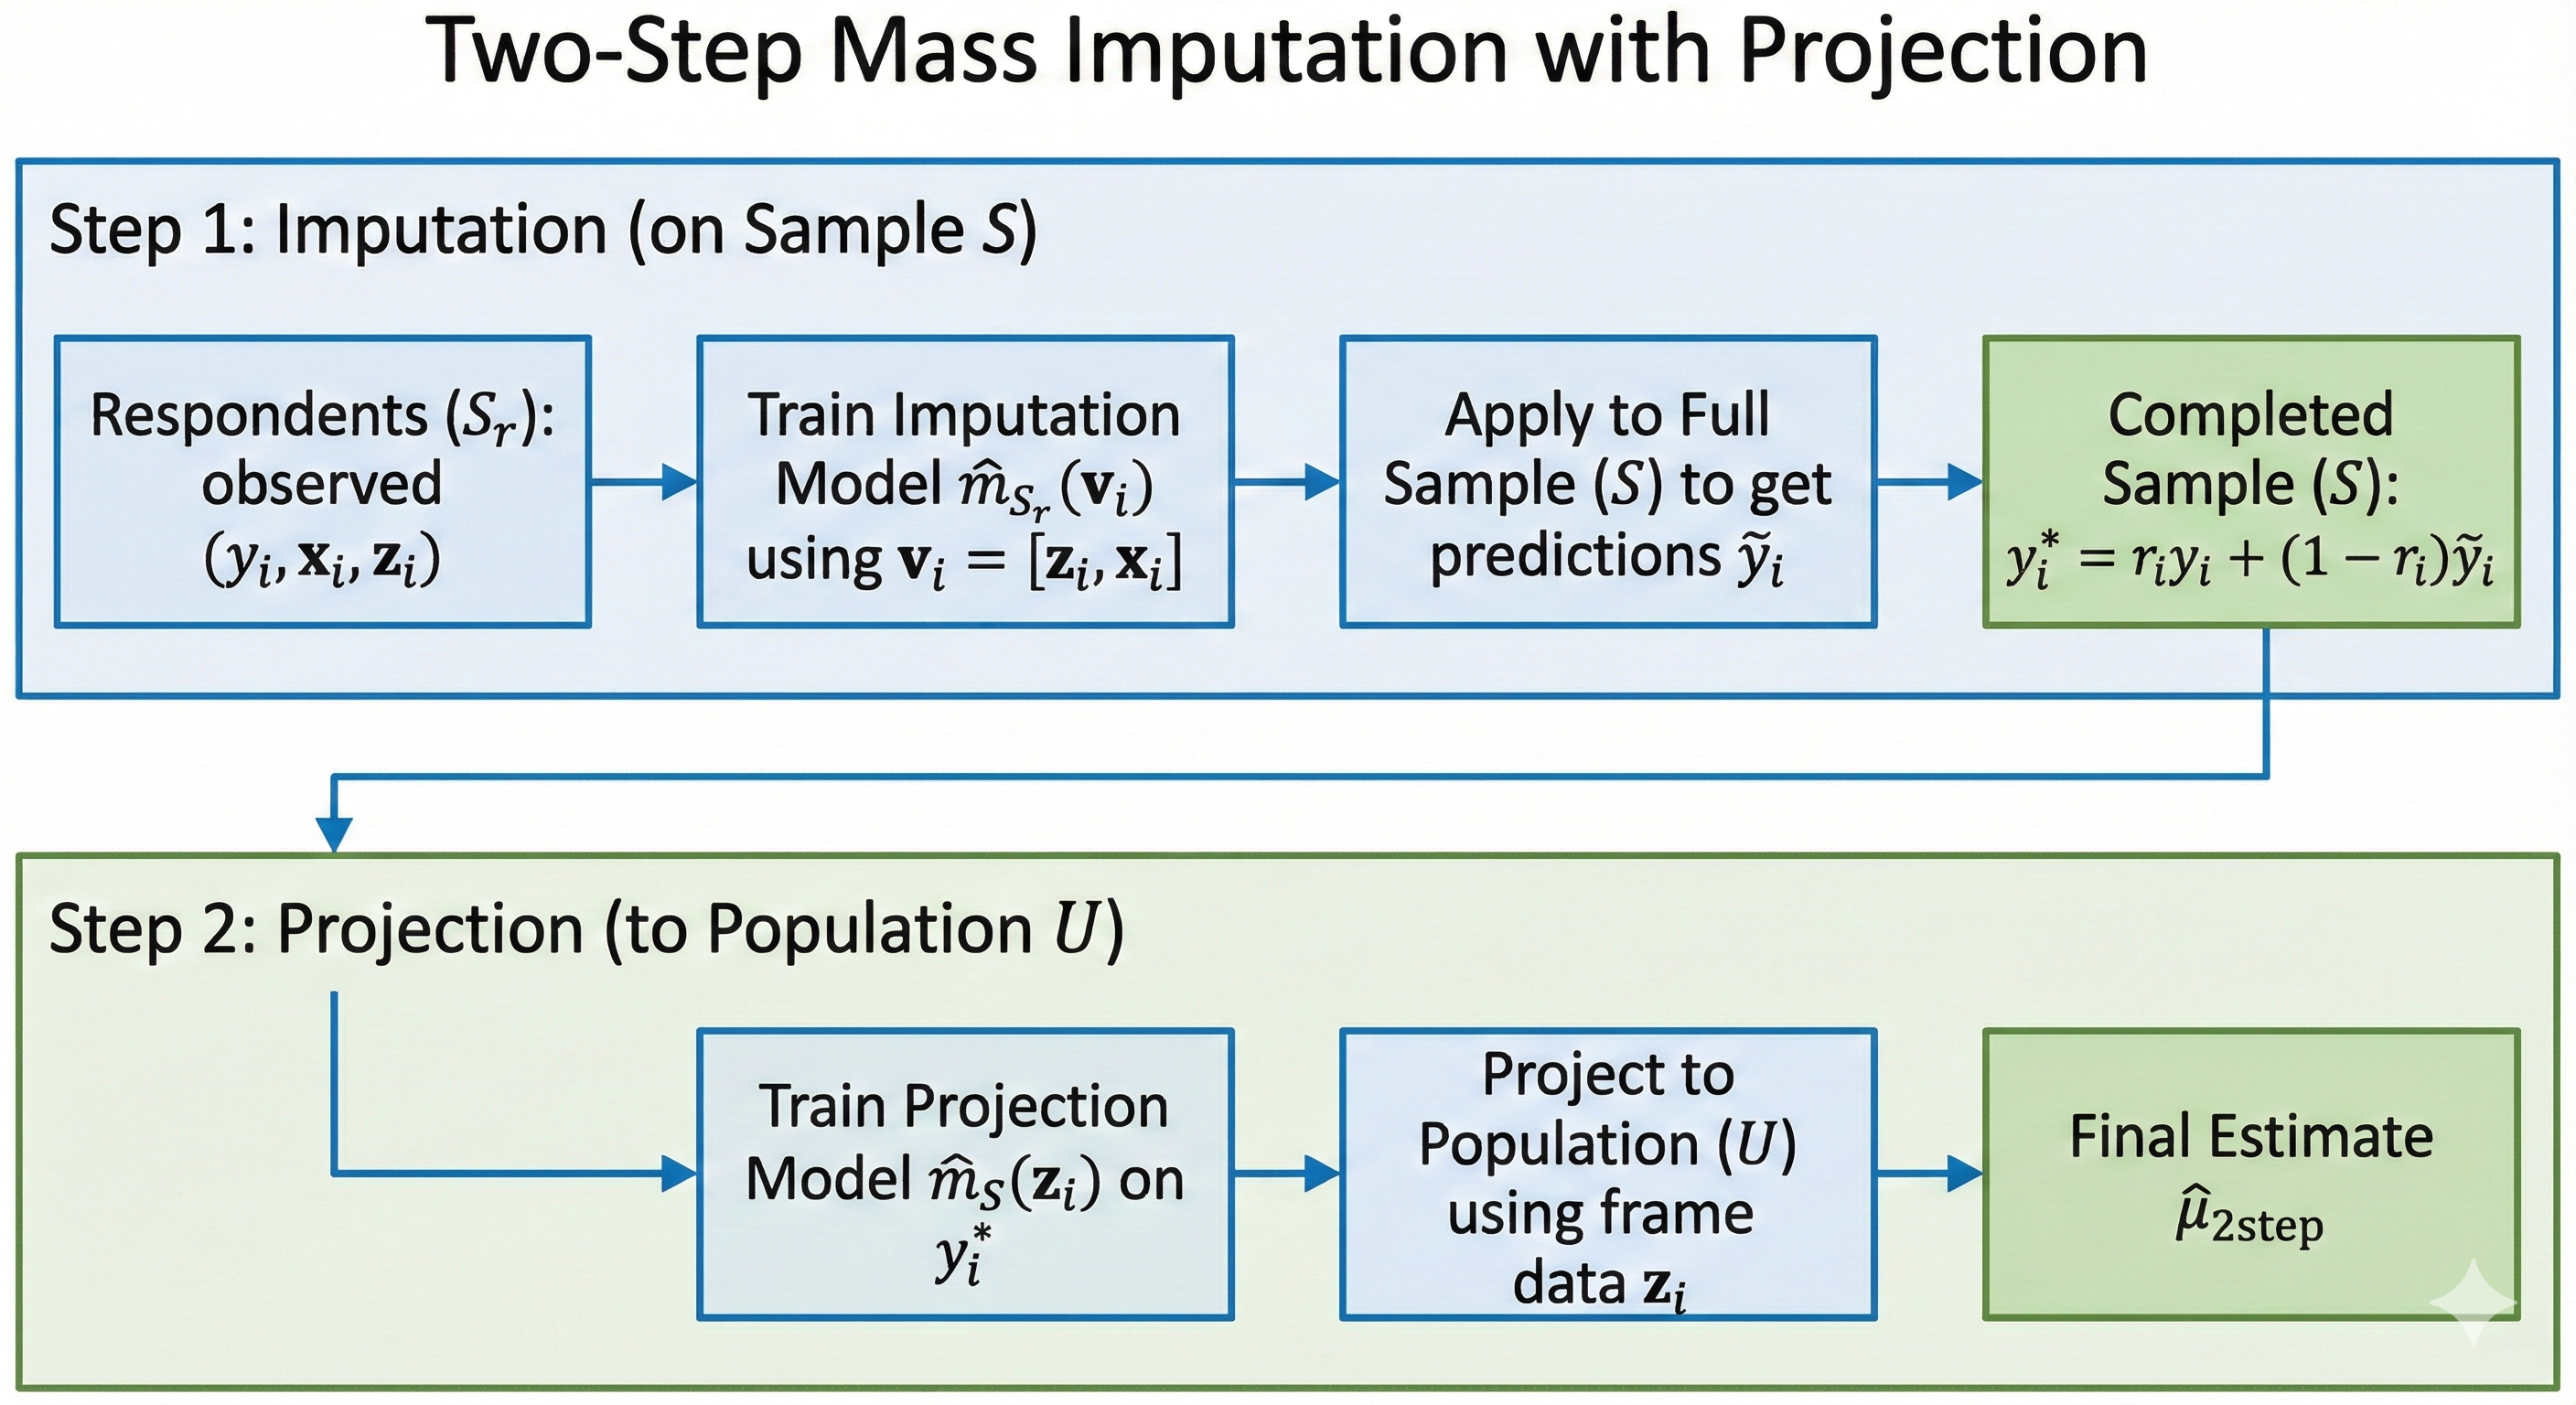
\includegraphics[width=0.8\textwidth]{paper/diagrams/3A.png}

% ------------------------------------------------- %
% ------------------ SCENARIO 4 ------------------- %
% ------------------------------------------------- %
\paragraph{Scenario 4: Historical Data and Pre-Trained Models.}

We now consider the specific case where the frame data $\mathbf{z}_i$ includes outcomes from a previous administrative period ($t-1$), such that $\mathbf{z}_i$ contains $y_i^{(t-1)}$. Additionally, we observe current-period auxiliary variables $\mathbf{x}_i$ for the sample $S$ which are not available on the frame. 

In this scenario, we rely on modeling assumptions (mass imputation) to handle missingness, reserving propensity score adjustments for the doubly robust framework in Scenario 5. We motivate the proposed estimator by first examining the limitations of two preliminary approaches.

\medskip
\noindent \textbf{1. The Naive Difference Estimator} \\
The simplest approach treats the previous period's outcome $y_i^{(t-1)}$ as a direct proxy for the current outcome $y_i$. Because current outcomes are only observed for respondents, a naive adjustment might be calculated over the respondent set $S_r$:
\begin{equation} \label{eq:s4_diff_naive}
\hat{\mu}_{\text{diff}} = \bar{Y}^{(t-1)} + \frac{1}{N}\sum_{i\in S_r}\frac{y_i - y_i^{(t-1)}}{\pi_i} 
\end{equation}
\noindent\textit{Critique:} This estimator is systematically biased. The summation term estimates the total change in outcome \textit{only for the respondent population}. It implicitly assumes that for the non-respondents (and the non-sampled population), the change in outcome is zero. It fails to utilize $\mathbf{x}_i$ to account for the heterogeneous evolution of $y_i$ across the population.

\medskip
\noindent \textbf{2. The Pre-trained Difference Estimator} \\
To reduce the variance of the difference estimator, one might employ a model $f_{\text{hist}}(\mathbf{z}_i)$ trained on historical trends (e.g., $y^{(t-1)} \sim \mathbf{z}^{(t-1)}$) to generate a baseline prediction. The estimator becomes:
\begin{equation} \label{eq:s4_diff_pretrain}
\hat{\mu}_{\text{Pre-train}}
= \frac{1}{N} \left(
  \sum_{i \in U} f_{\text{hist}}(\mathbf{z}_i)
  + \sum_{i \in S} \frac{r_i\bigl(y_i - f_{\text{hist}}(\mathbf{z}_i)\bigr)}{\pi_i}
\right)
\end{equation}
\noindent\textit{Critique:} While this method leverages the frame to stabilize the projection term (the first summand), the bias correction (the second summand) is still restricted to the respondent set $S_r$. If the relationship between $y_i$ and $\mathbf{z}_i$ has drifted due to factors associated with $\mathbf{x}_i$, and response depends on $\mathbf{x}_i$, the residual term computed over $S_r$ will be a biased estimate of the true population residual.

\medskip
\noindent \textbf{3. The Proposed Hist-PPD Estimator} \\
Finally, we propose the \textbf{Hist-PPD Estimator}, which adapts the Mass Imputation framework (Scenario 3) to this temporal context. 

We retain the historical function $f_{\text{hist}}(\mathbf{z}_i)$ for the population projection. However, to account for systematic evolution captured by current auxiliaries, we calculate the residuals using the \textit{completed} data vector $y_i^\star$ (as defined in Scenario 3), which contains imputed values $\hat{m}(\mathbf{v}_i)$ for non-respondents.

Crucially, because $y_i^\star$ is available for all sampled units, the residual adjustment is computed over the \textit{full sample} $S$, utilizing the sample design weights to project the residuals to the population:

\begin{equation} \label{eq:s4_hist_ppd}
\hat{\mu}_{\text{Hist-PPD}} = \frac{1}{N} \left( \underbrace{\sum_{i \in U} f_{\text{hist}}(\mathbf{z}_i)}_{\text{Population Projection}} + \underbrace{\sum_{i \in S} \frac{y_i^\star - f_{\text{hist}}(\mathbf{z}_i)}{\pi_i}}_{\text{Sample-based Adjustment}} \right) 
\end{equation}

This formulation ensures that:
\begin{enumerate}
    \item The historical model $f_{\text{hist}}$ provides the primary signal structure (low variance).
    \item The mass-imputed residuals $y_i^\star$ correct for temporal drift using the full sample information $S$, rather than the restricted respondent set $S_r$.
\end{enumerate}


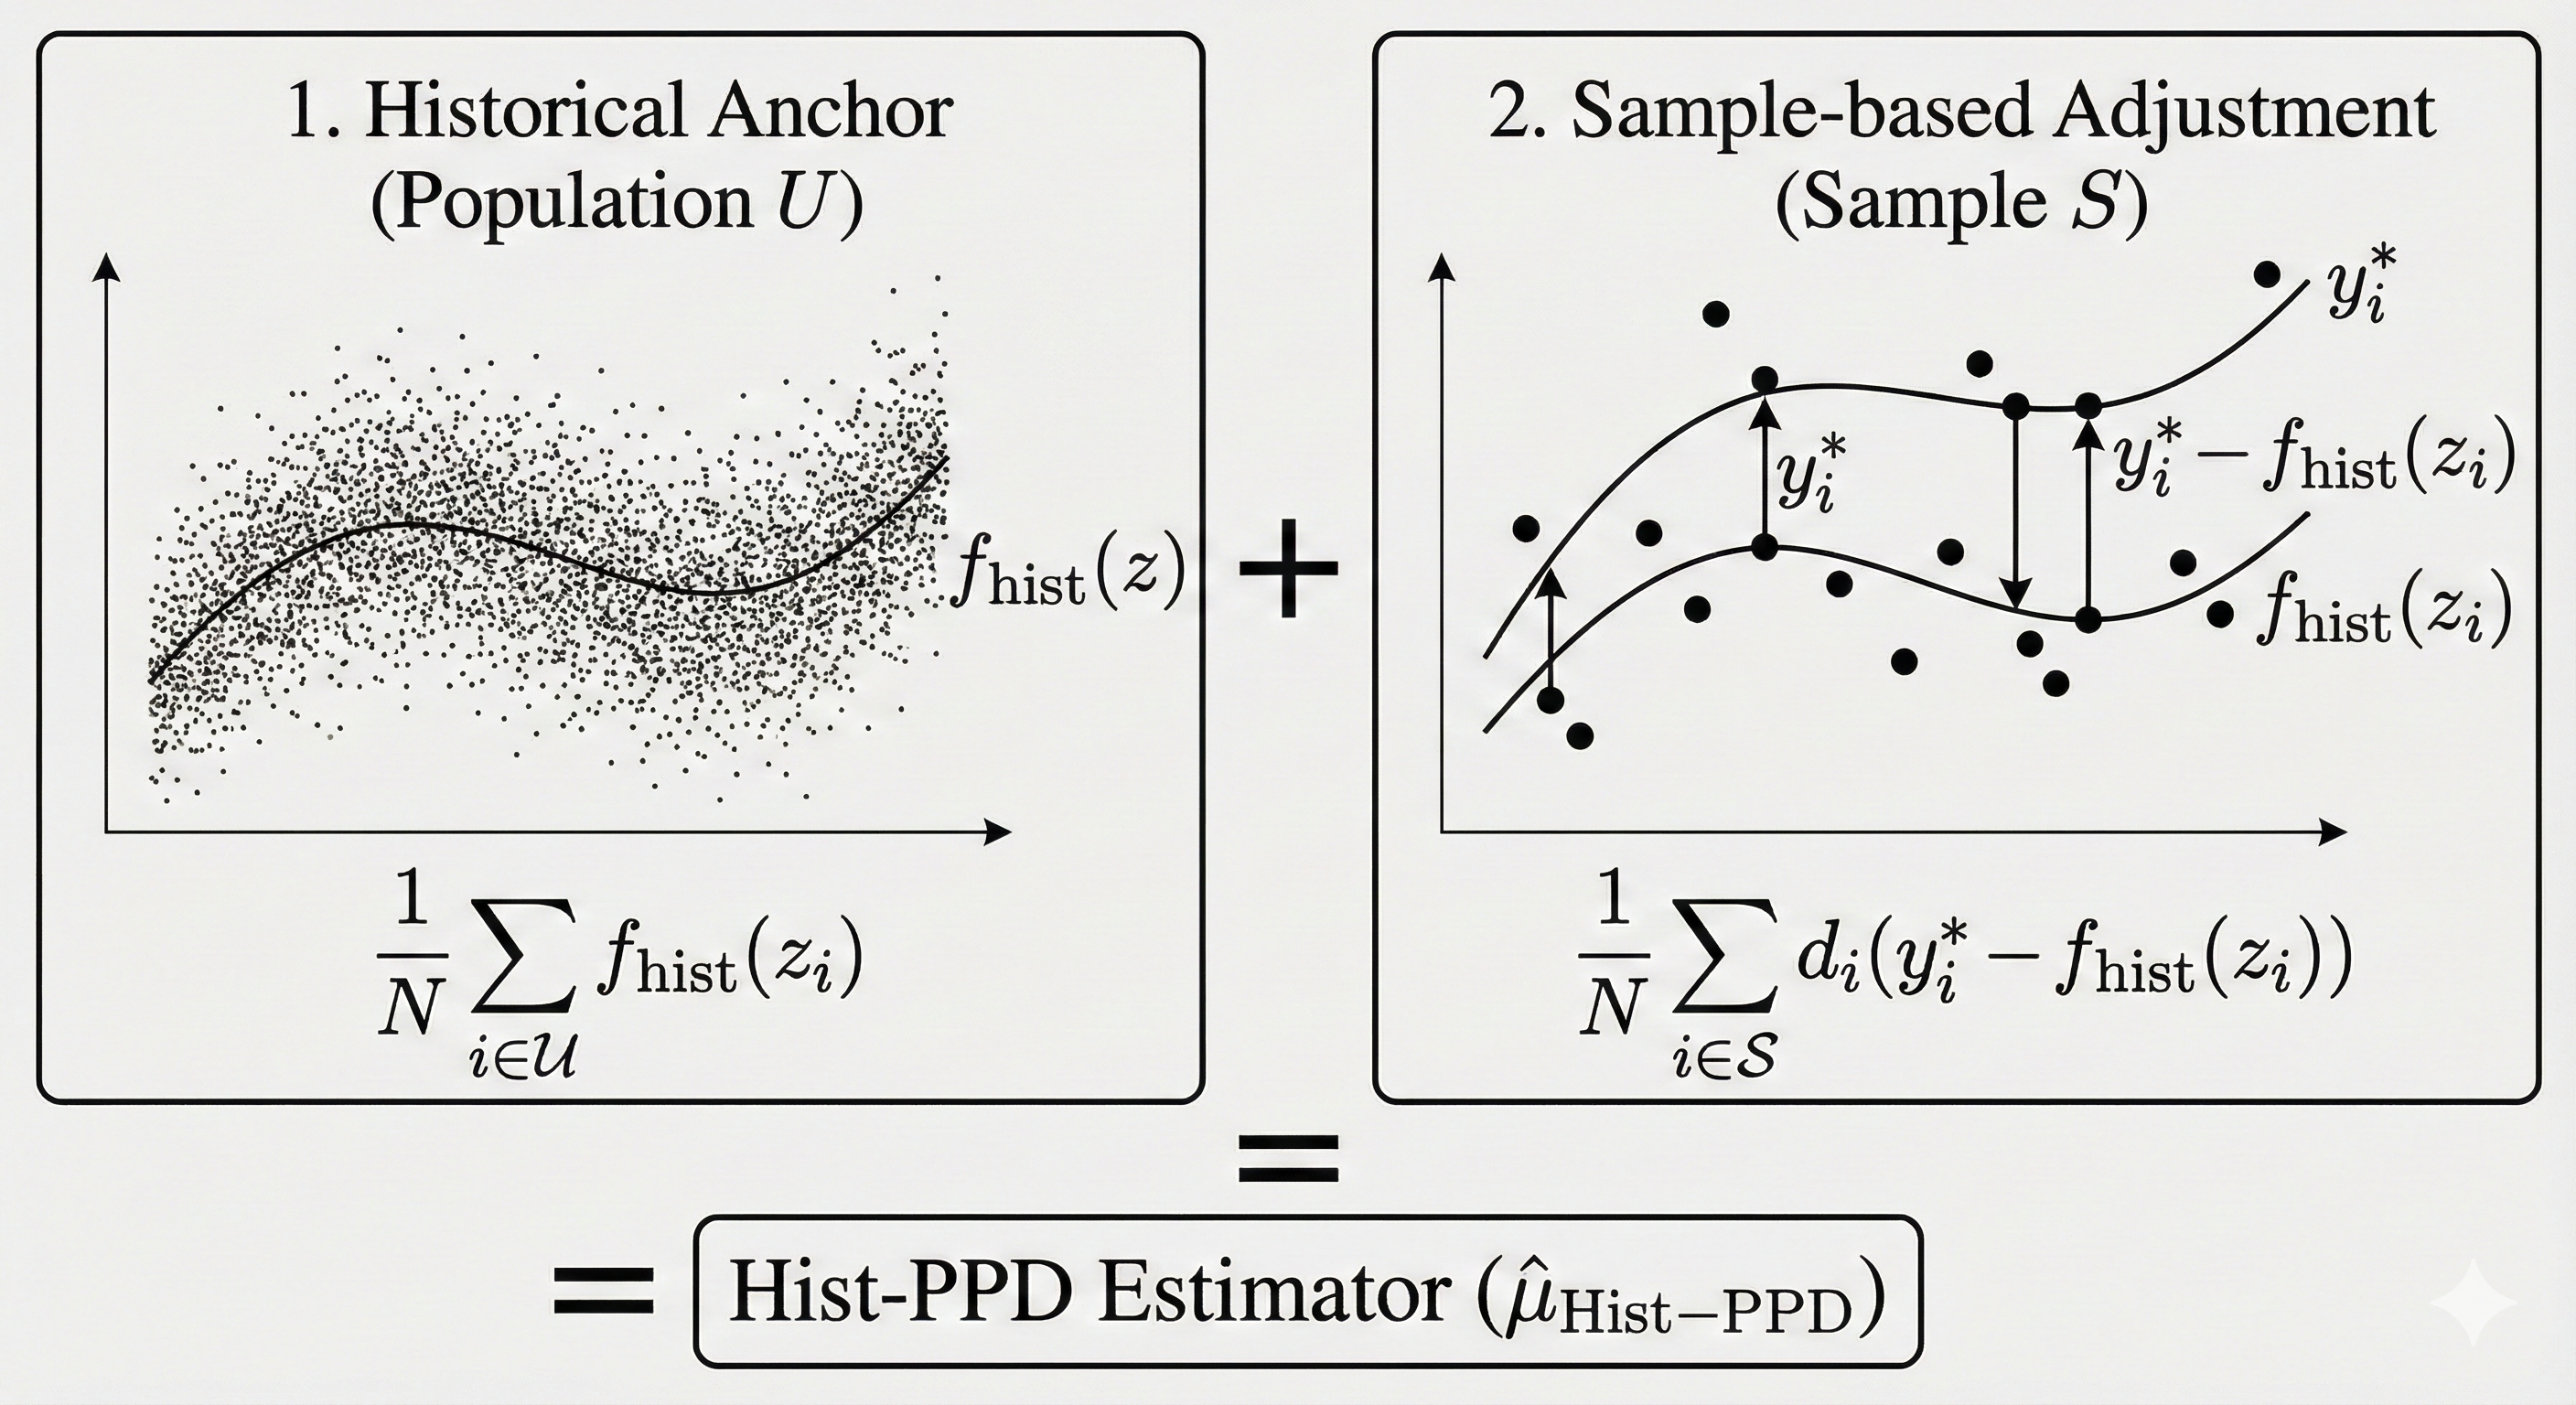
\includegraphics[width=0.8\textwidth]{paper/diagrams/Scenario4.png}

% ------------------------------------------------- %
% ------------------ SCENARIO 5 ------------------- %
% ------------------------------------------------- %
\paragraph{Scenario 5: Robust Integration (The Hist-PPD-DR Estimator).}
While the Hist-PPD estimator (Scenario 4) incorporates historical anchors and current signals, it relies heavily on the imputation model $\tilde{y}_i$ being an unbiased proxy for $y_i$. To safeguard against model misspecification (e.g., if the relationship between current signal $\mathbf{x}_i$ and outcome $y_i$ has drifted in a complex way), we apply a doubly robust correction.

This estimator applies the established doubly robust model-calibration framework \parencite[e.g.,]{kim_rao_2012_biometrika} to the historical setting. It augments the mass imputation estimator with an inverse-probability weighting (IPW) correction based on the response propensity $\hat{p}_i$.

\medskip
\noindent\emph{Estimator Formula.}
Let $\tilde{y}_i = \hat{m}_{S_r}(\mathbf{v}_i)$ be the predicted value from the imputation model using current signals, and let $f_{\text{hist}}(\mathbf{z}_i)$ be the historical projection. The robust estimator is:

\begin{equation} \label{eq:s5_hist_ppd_dr}
\hat{\mu}_{\text{Hist-PPD-DR}} = \frac{1}{N} \left( 
    \sum_{i\in U} f_{\text{hist}}(\mathbf{z}_i)
    \;+\; 
    \sum_{i\in S} \frac{1}{\pi_i} \Bigl\{\tilde{y}_i - f_{\text{hist}}(\mathbf{z}_i)\Bigr\}
    \;+\; 
    \sum_{i\in S} \frac{r_i}{\pi_i \hat{p}_i}\,\Bigl(y_i - \tilde{y}_i\Bigr)
\right)
\end{equation}

\noindent We can interpret this estimator by decomposing it into three distinct roles:

\[
\hat{\mu}_{\text{Hist-PPD-DR}} = \frac{1}{N} \left( 
    \underbrace{\sum_{i\in U} f_{\text{hist}}(\mathbf{z}_i)}_{\text{Historical Anchor}}
    \;+\; 
    \underbrace{\sum_{i\in S} \frac{1}{\pi_i} \Bigl\{\tilde{y}_i - f_{\text{hist}}(\mathbf{z}_i)\Bigr\}}_{\text{Model Shift (History } \to \text{ Current)}}
    \;+\; 
    \underbrace{\sum_{i\in S_r} \frac{1}{\pi_i \hat{p}_i}\Bigl(y_i - \tilde{y}_i\Bigr)}_{\text{Bias Correction (Residuals)}}
\right)
\]

\medskip
\noindent\emph{Properties and Sanity Checks.}
\begin{itemize}
    \item \textbf{Double Robustness:} The estimator is consistent for the population mean if \emph{either}:
    \begin{enumerate}
        \item The outcome model is correctly specified ($E[y_i|\mathbf{x}_i] \approx \tilde{y}_i$), \textbf{OR}
        \item The response propensity model is correctly specified ($\Pr(r_i=1|\mathbf{x}_i) \approx \hat{p}_i$).
    \end{enumerate}
    
    \item \textbf{Reduction to Mass Imputation (Scenario 4):} If we ignore the propensity weights (set $\hat{p}_i=1$) and assume the imputation residuals sum to zero over the sample, this collapses to $\hat{\mu}_{\text{Hist-PPD}}$.
    
    \item \textbf{Complete Response:} If $r_i \equiv 1$ (no missing data), the bias correction term $\sum (y_i - \tilde{y}_i)$ vanishes (in expectation), and the estimator collapses to the standard Difference Estimator using $f_{\text{hist}}$.
    
    \item \textbf{No History:} If $f_{\text{hist}} \equiv 0$, the estimator simplifies to the classic AIPW (Doubly Robust) estimator (Equation \ref{eq:s1_dr}).
\end{itemize}


\begin{table}[htbp]
\centering
\caption{Comparison of Estimators: Training Data sources, Prediction Targets, and Auxiliary Usage. Note the distinction in Mass Imputation between the model trained on respondents ($\hat{m}_{S_r}$) and the model trained on the completed sample ($\hat{m}_S$).}
\label{tab:estimators_comparison}
\renewcommand{\arraystretch}{1.3} % Adds breathing room between rows
\resizebox{\textwidth}{!}{% Resizes table to fit text width if necessary
\begin{tabular}{@{} l l l l l @{}}
\toprule
\textbf{Estimator} & \textbf{Key Component} & \textbf{Training Set} (Learns $\beta$) & \textbf{Prediction Target} (Gets $\hat{y}$) & \textbf{Auxiliaries Used} \\ 
\midrule

% Row 1: Imputation
\textbf{1. Imputation} & 
$\hat{m}_{S_r}(\mathbf{x}_i)$ & 
Respondents ($S_r$) & 
Missing Sample ($S_m$) & 
Sample ($\mathbf{x}$) \\

% Row 2: NWA
\textbf{2. NWA (IPW)} & 
$\hat{p}_i(\mathbf{v}_i)$ & 
Full Sample $S$ (Response Flag) & 
Respondents ($S_r$) & 
Sample ($\mathbf{x}$) \\

% Row 3: GREG
\textbf{3. Std. GREG} & 
$\hat{m}_{S_r}(\mathbf{z}_i)$ & 
Respondents ($S_r$) & 
Population ($U$) & 
Frame ($\mathbf{z}$) \\

\midrule

% Row 4: Mass Imputation (Split into two steps for clarity)
\textbf{4. Mass Imputation} & & & & \\
\hspace{3mm} \textit{Step 1: Impute} & 
$\hat{m}_{S_r}(\mathbf{v}_i)$ & 
Respondents ($S_r$) & 
Full Sample ($S$) & 
Rich Sample ($\mathbf{x}, \mathbf{z}$) \\
\hspace{3mm} \textit{Step 2: Project} & 
$\hat{m}_{S}(\mathbf{z}_i)$ & 
\textbf{Completed Sample} ($S$) & 
Population ($U$) & 
Frame ($\mathbf{z}$) \\

\midrule

% Row 5: Hist-PPD
\textbf{5. Hist-PPD} & 
$f_{\text{hist}}(\mathbf{z}_i)$ & 
\textbf{Historical Data} ($t-1$) & 
Population ($U$) & 
History ($\mathbf{z}$) \\

% Row 6: Hist-PPD-DR
\textbf{6. Hist-PPD-DR} & 
$f_{\text{hist}}$ + $\hat{m}_{S_r}$ & 
History ($t-1$) \textbf{\&} Respondents ($S_r$) & 
Population ($U$) & 
\textbf{All} ($\mathbf{x}, \mathbf{z}, \text{History}$) \\

\bottomrule
\end{tabular}%
}
\end{table}


% ------------------------------------------------- %
% -------------- MODEL SPECIFICATION -------------- %
% ------------------------------------------------- %
\section{Model Specification}
\label{sec:model_spec}


To implement the Hist-PPD-DR estimator defined in Equation \eqref{eq:s5_hist_ppd_dr}, we must specify two distinct working models: the outcome model $m_S(\mathbf{v}_i)$ used for mass imputation, and the response probability model $\hat{p}_i(\mathbf{v}_i)$ used for propensity weighting.

Throughout, we adopt the standard Missing at Random (MAR) assumption for item nonresponse: $r_i \perp y_i \mid \mathbf v_i$, where $\mathbf v_i = [\mathbf z_i,\mathbf x_i]$ collects the frame and sample auxiliaries observed for every sampled unit. Under MAR it is not contradictory that the same predictor vector $\mathbf v_i$ drives both the outcome model $m_S(\mathbf v_i)$ used for imputation and the response model $\rho(\mathbf v_i) = \Pr(r_i=1 \mid \mathbf v_i)$ used for weighting. Intuitively, $\mathbf v_i$ is allowed to explain both how large $y_i$ tends to be and how likely unit $i$ is to respond; MAR only rules out any remaining dependence of $r_i$ on the unobserved part of $y_i$ once $\mathbf v_i$ is fixed. This is precisely the setup used in the survey–sampling literature on nonresponse adjustment: doubly robust and model–calibration estimators are built from one regression of $y$ on $\mathbf v_i$ and one regression of $r_i$ on $\mathbf v_i$, fitted on the same set of auxiliaries that are available for all units in the sample \parencite[e.g.,]{little_rubin_2002_samd,kim_haziza_2014_sinica,Haziza2017,kim_rao_2012_biometrika}. In our application, we follow this principle by taking $\mathbf v_i=[\mathbf z_i,\mathbf x_i]$ as the common predictor set for both the XGBoost imputation model and the logistic propensity model.


Recent literature in survey sampling emphasizes that while Double Robustness protects against the misspecification of one model, the finite-sample performance of the estimator depends heavily on the stability and predictive power of these models \parencite{Haziza2017}. Consequently, we adopt a hybrid modeling strategy that leverages the strengths of machine learning for prediction and the stability of parametric estimation for weighting.

\subsection{Imputation Model: Gradient Boosted Trees (XGBoost)}

\begin{enumerate}
    \item \textbf{Automatic Interaction Detection:} Unlike linear models, which require explicit specification of interaction terms (e.g., $\mathbf{x}_i \times \mathbf{z}_i$), XGBoost automatically learns complex non-linear interactions between the frame and sample data.
    \item \textbf{Robustness to Skewness:} Survey data often follow heavy-tailed distributions (e.g., Gamma-like revenue data). Tree-based methods are invariant to monotonic transformations of the predictors and are less sensitive to outliers in the covariate space than linear projection methods.
    \item \textbf{Regularization:} XGBoost includes both $L_1$ and $L_2$ regularization terms in its objective function, preventing overfitting even when the number of sample predictors $p_x$ is large relative to the sample size $n$.
\end{enumerate}

\subsection{Propensity Score Model: The Parametric Score Method}

For the propensity score estimation $\hat{p}_i$, we employ a parametric logistic regression model estimated via the \textbf{Score Method} (Maximum Likelihood), rather than a machine learning classifier. While machine learning methods like XGBoost are powerful classifiers, they are often ill-suited for propensity weighting in finite population inference. A known issue with boosting or random forests in this context is ``perfect separation,'' where the model assigns probabilities close to 0 or 1. In a weighting context (Scenario 1 and 3), this results in extreme weights ($\hat{p}_i^{-1}$) that can destabilize the estimator and drastically inflate variance. In contrast, the Score Method (Logistic Regression) provides two critical statistical properties required for robust weighting \parencite{KimHaziza2014}:

\begin{enumerate}
    \item \textbf{Calibration Constraints:} The maximum likelihood estimator $\hat{\boldsymbol{\alpha}}$ for the logistic model solves the score equations:
    \begin{equation} \label{eq:score_eqn}
        \sum_{i \in S} \left( r_i - \frac{1}{1 + \exp(-\mathbf{v}_i^T \boldsymbol{\alpha})} \right) \mathbf{v}_i = \mathbf{0}
    \end{equation}
    This implies that the residuals sum to zero over the sample space. As noted by \parencite{Haziza2017}, this inherent balancing property ensures that the estimated weights effectively align the covariate distributions of the respondents and the sample, a property not guaranteed by standard machine learning classifiers.
    
    \item \textbf{Boundedness:} The logistic link function produces smooth probabilities strictly bounded away from 0 and 1 (assuming no complete separation), resulting in a more stable distribution of weights and lower variance for the final estimator.
\end{enumerate}

Therefore, our simulation utilizes XGBoost for $m_S(\cdot)$ to maximize predictive accuracy, and Logistic Regression for $\rho(\cdot)$ to ensure stability and calibration of the weights.




% ------------------------------------------------- %
% ------------------- NEW SECTION ------------------- %
% ------------------------------------------------- %

%% Variance estimation
\section{Variance Estimation}

A major challenge in using the estimator proposed in Scenario 3 is variance estimation. Standard variance formulas (e.g., Horvitz-Thompson variance) treat the completed values $y_i^\star$ as if they were observed values. This leads to the ``naive variance estimation'' problem, where the uncertainty associated with the imputation model $\hat{m}_{S_{r}}(\cdot)$ is ignored, resulting in standard errors that are too small and confidence intervals that have poor coverage \parencite{kim_rao_2012_biometrika}.

To properly account for both the sampling design and the uncertainty in the imputation mechanism, we recommend a replication-based approach, specifically the bootstrap.

\paragraph{The Bootstrap for Mass Imputation.}
To estimate the variance of our estimators, we employ a bootstrap procedure that captures the variability of the model fitting process. The procedure is as follows:

\begin{enumerate}
    \item \textbf{Generate Replicates:} Draw $B$ bootstrap samples $S^{(b)}$ from the original sample $S$ using the design weights (e.g., using the rescaling bootstrap for complex designs).
    \item \textbf{Re-Impute:} For each bootstrap sample $b = 1, \dots, B$:
    \begin{itemize}
        \item Refit the imputation model $\hat{m}_{S_{r}}^{(b)}(\mathbf{v}_i)$ using only the respondents in the bootstrap replicate $S_r^{(b)}$.
        \item Generate new imputed values $\tilde{y}_i^{(b)}$ for the non-respondents in that replicate.
        \item Refit the projection model $\hat{m_S}^{(b)}(\mathbf{z}_i)$ on the completed bootstrap sample (unless utilizing a fixed historical model $f_{\text{hist}}$, which remains constant).
    \end{itemize}
    \item \textbf{Calculate Estimate:} Compute the estimator $\hat{\mu}^{(b)}$ for each replicate.
\end{enumerate}

The variance estimator is then the empirical variance of the $B$ bootstrap estimates:
\begin{equation} \label{eq:boot_var}
\widehat{V}(\hat{\mu}_{\text{PPD-DR}}) = \frac{1}{B-1} \sum_{b=1}^B \left( \hat{\mu}^{(b)} - \bar{\hat{\mu}} \right)^2
\end{equation}
where $\bar{\hat{\mu}}$ is the mean of the bootstrap replicates. This method is asymptotically consistent and automatically captures the additional variance introduced by the imputation and projection steps.






\section{Simulation}


\subsection{Bootstrap implementation for each estimator}

For variance estimation and for computing coverage in the simulation study, we use a design based bootstrap. Let $S$ denote the original sample, with design weights $d_i = 1/\pi_i$, and let $S_r$ and $S_m$ denote the respondent and missing subsets. Let $U$ denote the finite population. Throughout the bootstrap the population $\{(y_i,\mathbf{x}_i,\mathbf{z}_i): i\in U\}$, the frame auxiliaries $\mathbf{z}_i$, and the historically trained prediction function $f_{\text{hist}}(\mathbf{z}_i)$ are treated as fixed and known.

For $b = 1,\dots,B$ we draw a bootstrap sample $S^{(b)}$ from $S$ using a standard design based bootstrap (for example, the rescaling bootstrap for complex designs). The resulting rescaled weights are written $d_i^{(b)}$ for $i\in S^{(b)}$, and $S^{(b)}_r$ denotes the respondent set in the $b$th bootstrap sample. On each bootstrap sample we refit all models that, in practice, would be estimated from the realized sample, and then recompute the estimator of interest. The bootstrap variance for an estimator $\hat\mu$ is
\[
\widehat{\mathrm{Var}}_B(\hat\mu)
  = \frac{1}{B-1}\sum_{b=1}^B\Bigl(\hat\mu^{(b)} - \bar\mu_B\Bigr)^2,
\qquad
\bar\mu_B = \frac{1}{B}\sum_{b=1}^B \hat\mu^{(b)}.
\]
Below we summarize, estimator by estimator, which components are re-estimated inside each bootstrap replicate, and which are held fixed.

\paragraph{Naive Horvitz--Thompson (respondents only).}
This estimator ignores nonresponse and auxiliary information. In each bootstrap sample $S^{(b)}$ we compute
\[
\hat\mu_{\text{naive}}^{(b)}
  = \frac{1}{N}\sum_{i\in S_r^{(b)}} d_i^{(b)} y_i.
\]
No model is fitted in this case; only the design weights are rescaled by the bootstrap.

\paragraph{Nonresponse weighting only (NWA / IPW).}
This estimator uses only a propensity model for response. For each bootstrap sample $S^{(b)}$:
\begin{enumerate}
  \item Fit the parametric propensity model $\hat p_i^{(b)} = \Pr(r_i=1\mid \mathbf{v}_i)$ by logistic regression of $r_i$ on $\mathbf{v}_i = [\mathbf{z}_i,\mathbf{x}_i]$ using all units in $S^{(b)}$.
  \item Compute the IPW estimator
  \[
  \hat\mu_{\text{NWA}}^{(b)}
    = \frac{1}{N}\sum_{i\in S_r^{(b)}} \frac{d_i^{(b)}}{\hat p_i^{(b)}}\,y_i.
  \]
\end{enumerate}
Thus the propensity model is re-estimated in every bootstrap replicate; the population and frame data remain fixed.

\paragraph{Standard nonresponse GREG / Hist-GREG.}
This estimator uses a regression of $y_i$ on the frame auxiliaries $\mathbf{z}_i$ together with a propensity model for response. For each bootstrap sample $S^{(b)}$:
\begin{enumerate}
  \item Fit the outcome model $\hat m_{S_r^{(b)}}(\mathbf{z}_i)$ on the respondents $S_r^{(b)}$ (for example, a linear or generalized linear regression of $y_i$ on $\mathbf{z}_i$).
  \item Fit the propensity model $\hat p_i^{(b)} = \Pr(r_i=1\mid \mathbf{v}_i)$ on $S^{(b)}$ by logistic regression of $r_i$ on $\mathbf{v}_i = [\mathbf{z}_i,\mathbf{x}_i]$.
  \item Evaluate $\hat m_{S_r^{(b)}}(\mathbf{z}_i)$ for all $i\in U$ using the frame data, and compute
  \[
  \hat\mu_{\text{GREG}}^{(b)}
    = \frac{1}{N}\left(
        \sum_{i\in U} \hat m_{S_r^{(b)}}(\mathbf{z}_i)
        + \sum_{i\in S_r^{(b)}} \frac{d_i^{(b)}}{\hat p_i^{(b)}}
          \bigl\{y_i - \hat m_{S_r^{(b)}}(\mathbf{z}_i)\bigr\}
      \right).
  \]
\end{enumerate}
Both the regression of $y$ on $\mathbf{z}$ and the response propensity model are refit in each bootstrap replicate; the frame $\{\mathbf{z}_i : i\in U\}$ is treated as fixed.

\paragraph{Two-step mass imputation and Hist-PPD.}
The mass imputation class uses a rich outcome model fitted on respondents to complete the sample, followed by a projection based on frame information. In the generic two-step projection estimator (Scenario~3) we have:
\begin{enumerate}
  \item Fit a rich imputation model $\hat m_{S_r^{(b)}}(\mathbf{v}_i)$ on $S_r^{(b)}$ and form completed outcomes
  \[
  y_i^{\star (b)} = r_i y_i + (1-r_i)\,\hat m_{S_r^{(b)}}(\mathbf{v}_i),
  \qquad i\in S^{(b)}.
  \]
  \item Fit a coarser projection model $\hat m_{S^{(b)}}(\mathbf{z}_i)$ on the completed sample $\{(y_i^{\star (b)},\mathbf{z}_i): i\in S^{(b)}\}$.
  \item Use the projection estimator
  \[
  \hat\mu_{2\text{step}}^{(b)}
    = \frac{1}{N}\left(
        \sum_{i\in U} \hat m_{S^{(b)}}(\mathbf{z}_i)
        + \sum_{i\in S^{(b)}} d_i^{(b)}
          \bigl\{y_i^{\star (b)} - \hat m_{S^{(b)}}(\mathbf{z}_i)\bigr\}
      \right).
  \]
\end{enumerate}
Both the rich imputation model and the projection model are re-estimated in every bootstrap replicate; the frame $\mathbf{z}_i$ is fixed.

The Hist-PPD estimator (Scenario~4) is a special case where the projection term is supplied by the historical function $f_{\text{hist}}(\mathbf{z}_i)$. In each bootstrap replicate we still refit the rich imputation model $\hat m_{S_r^{(b)}}(\mathbf{v}_i)$ and form $y_i^{\star (b)}$ as above, but we treat $f_{\text{hist}}(\cdot)$ as fixed and compute
\[
\hat\mu_{\text{Hist-PPD}}^{(b)}
  = \frac{1}{N}\left(
      \sum_{i\in U} f_{\text{hist}}(\mathbf{z}_i)
      + \sum_{i\in S^{(b)}} d_i^{(b)}
        \bigl\{y_i^{\star (b)} - f_{\text{hist}}(\mathbf{z}_i)\bigr\}
    \right).
\]
Thus, for Hist-PPD the only model that is re-estimated inside the bootstrap is the imputation model on the respondents; the historical anchor $f_{\text{hist}}$ is reused across all bootstrap replicates.

\paragraph{Hist-PPD-DR (Scenario~5, proposed).}
The doubly robust estimator combines the historical anchor, the mass imputation signal, and a propensity based bias correction. In each bootstrap sample $S^{(b)}$:
\begin{enumerate}
  \item Fit the rich imputation model $\hat m_{S_r^{(b)}}(\mathbf{v}_i)$ on $S_r^{(b)}$ and compute the predicted values
  \[
  \tilde y_i^{(b)} = \hat m_{S_r^{(b)}}(\mathbf{v}_i), \qquad i\in S^{(b)}.
  \]
  \item Fit the propensity model $\hat p_i^{(b)} = \Pr(r_i = 1 \mid \mathbf{v}_i)$ by logistic regression of $r_i$ on $\mathbf{v}_i$ using all units in $S^{(b)}$.
  \item Evaluate $f_{\text{hist}}(\mathbf{z}_i)$ for all $i\in U$ (using the fixed historical model) and compute
  \[
  \hat{\mu}_{\text{Hist-PPD-DR}}^{(b)}
    = \frac{1}{N}\left(
        \sum_{i\in U} f_{\text{hist}}(\mathbf{z}_i)
        + \sum_{i\in S^{(b)}} d_i^{(b)}
          \bigl\{\tilde y_i^{(b)} - f_{\text{hist}}(\mathbf{z}_i)\bigr\}
        + \sum_{i\in S_r^{(b)}} \frac{d_i^{(b)}}{\hat p_i^{(b)}}
          \bigl\{y_i - \tilde y_i^{(b)}\bigr\}
      \right),
  \]
  which is the bootstrap analogue of equation~\eqref{eq:s5_hist_ppd_dr}.
\end{enumerate}
In this case both working models are re-estimated for every bootstrap replicate: the outcome model used for mass imputation and the propensity model for response. The historical function $f_{\text{hist}}$ and the frame data remain fixed.

This estimator by estimator description makes explicit which parts of each procedure are treated as random in the bootstrap. In particular, whenever an estimator would involve fitting a regression or propensity model in practice, that model is refit inside every bootstrap replicate; fixed frame information and historical models are not resampled.

\subsection{Simulation Setup}
We employ a four-step data generation process to create a finite population, draw samples, induce non-response, and compute estimates. We repeat this process $K=2,000$ times to approximate the sampling distribution of the estimators.

\paragraph{Data Generation Process.}
We generate a finite population $U$ of size $N=10,000$. Following the simulation designs of \textcite{Haziza2017}, we utilize Gamma distributions to mimic the right-skewed nature of business survey data (e.g., revenue or production).

\begin{itemize}
    \item \textbf{Historical Administrative Data ($z_i$):} 
    We generate a historical variable $z_i$ (representing, for example, previous census revenue) from a Gamma distribution with shape $\alpha=2$ and scale $\beta=10$:
    \[ z_i \sim \text{Gamma}(2, 10) \]
    This results in a strictly positive, right-skewed distribution with a mean of 20, typical of economic populations.
    
    \item \textbf{Current Signal ($x_i$):} 
    We generate the current signal $x_i$ (e.g., a real-time auxiliary signal) as a function of the history, subject to drift. We use an additive error structure with a positive distribution to ensure $x_i$ remains strictly positive:
    \[ x_i = 0.8 z_i + \epsilon_{x,i} \]
    where $\epsilon_{x,i} \sim \text{Exponential}(5)$. This creates a strong positive correlation ($\rho \approx 0.7$) between the past and present, reflecting a stable but evolving population.
    
    \item \textbf{Outcome Variable ($y_i$):} 
    We generate the current outcome of interest $y_i$ as a function of both the historical anchor and the current signal:
    \[ y_i = 2 + 0.5 z_i + 1.5 x_i + \epsilon_{y,i} \]
    where $\epsilon_{y,i} \sim N(0, 5)$. This setup ensures that while history ($z_i$) is predictive, the current signal ($x_i$) contains unique, necessary information to capture the true outcome.
    
    \item \textbf{Sampling ($S$):} 
    From the population, we draw a probability sample $S$ of size $n=500$ using Simple Random Sampling (SRS).
    
    \item \textbf{Non-response ($r_i$):} 
    We introduce item non-response using a logistic propensity model. To simulate informative missingness often found in business surveys (where unit size affects response behavior), we model the response probability as a function of the current signal $x_i$:
    \[ \text{logit}(\Pr(r_i=1)) = -1 + 0.1 x_i \]
    This induces a Missing at Random (MAR) mechanism. Crucially, because response depends on $x_i$, and $y_i$ depends on $x_i$, the observed set of respondents is systematically biased. Estimators that fail to account for $x_i$ will therefore yield biased inference.
\end{itemize}


\subsection{Evaluation Metrics}

We assess the performance of each estimator using three standard statistical metrics. Let $\hat{\theta}_k$ be the estimate from the $k$-th simulation run and $\theta$ be the true population total.

We measure systematic error using Relative Bias (RB). Values close to 0\% indicate unbiasedness; generally, an absolute relative bias greater than 5\% is considered problematic in official statistics.
\[ \text{RB}(\hat{\theta}) = \frac{1}{K} \sum_{k=1}^{K} \left( \frac{\hat{\theta}_k - \theta}{\theta} \right) \times 100\% \]

We measure efficiency using Relative Root Mean Square Error (RRMSE), which captures the combined effect of bias and variance.
\[ \text{RRMSE}(\hat{\theta}) = \sqrt{ \frac{1}{K} \sum_{k=1}^{K} \left( \frac{\hat{\theta}_k - \theta}{\theta} \right)^2 } \times 100\% \]

Finally, we evaluate uncertainty quantification using the Coverage Rate (CR), 
\[ \text{CR} = \frac{1}{K} \sum_{k=1}^{K} \mathbbm{1}\{ \theta \in [\hat{\theta}_k \pm 1.96 \sqrt{\widehat{V}_k}] \} \]
defined as the proportion of simulation runs where the 95\% confidence interval contains the true population value. A valid estimator should have a coverage rate close to 95\%.

\subsection{Comparisons}

We compare five distinct estimators to isolate the contributions of historical data, current signals, and robust corrections:

\begin{enumerate}
    \item \textbf{Naive Estimator:} The standard Horvitz-Thompson estimator using only the respondents $S_r$. It ignores missingness and makes no use of auxiliary data.
    \item \textbf{Weighting Only (NWA):} The standard IPW estimator that adjusts for non-response using propensity scores $\hat{p}_i(x_i, z_i)$, but utilizes no outcome modeling (Scenario 1).
    \item \textbf{Standard Hist-GREG:} The classical generalized regression estimator using only historical data $z_i$ for the projection. It ignores the rich current signals $x_i$ inside the imputation model (Scenario 2).
    \item \textbf{Mass Imputation (Two-Step):} The projection estimator that uses current signals $x_i$ to impute missing values, but lacks the propensity score correction for double robustness (Scenario 3, also the Hist-PPD).
    
    
    \item \textbf{Hist-PPD-DR:} The proposed approach which integrates all available information. It uses $z_i$ for the population anchor, $x_i$ for mass imputation, and propensity weights for residual bias correction.
\end{enumerate}



\newpage
\begin{table}[htbp]
\centering
\scriptsize
\renewcommand{\arraystretch}{2.0}
\caption{Comprehensive Summary of Estimators for Item Nonresponse (Finite-Population Total)}
\label{tab:comprehensive_estimators}

\resizebox{\textwidth}{!}{%
\begin{tabular}{@{} p{2.5cm} p{5.5cm} p{1.5cm} p{2.2cm} p{3.0cm} p{2.5cm} @{}}
\toprule
\textbf{Estimator} & 
\textbf{Formula} ($\widehat{T}$) & 
\textbf{Respon-dents Only?} & 
\textbf{Model Required} & 
\textbf{Assumptions for Consistency} & 
\textbf{Key References} \\ 
\midrule

% 1. Naive
\textbf{Naïve} &
$\displaystyle \widehat{T}_{\text{naive}} = \frac{N}{\sum_{j \in S_r} d_j} \sum_{i \in S_r} d_i y_i$ &
Yes &
None &
MCAR &
\textcite{cochran_1977_sampling}; \textcite{little_rubin_2002_samd} \\

% 2. NWA / Propensity Weighting
\textbf{Propensity Weighting (NWA)} &
$\displaystyle \widehat{T}_{\text{NWA}} = \sum_{i \in S_r} \frac{d_i}{\hat{p}_i} y_i$ &
Yes &
Response $\hat{p}(\mathbf{v})$ &
MAR, Positivity, Correct $\hat{p}$ &
\textcite{little_1986_isr}; \textcite{kott_1994_jasa}; \textcite{robins_rotnitzky_zhao_1994_jasa} \\

% 3. Calibration / GREG
\textbf{Calibration / GREG} &
$\displaystyle \widehat{T}_{\text{reg}} = \sum_{i \in U} f(\mathbf{z}_i) + \sum_{i \in S_r} \frac{d_i}{\hat{p}_i} (y_i - f(\mathbf{z}_i))$ \newline
\textit{(Note: Standard GREG often assumes $\hat{p}_i=1$)} &
Yes &
Outcome $f(\mathbf{z})$ &
Aux $\mathbf{z}$ predictive of $y$; Either correct $f(\mathbf{z})$ OR correct $\hat{p}$ &
\textcite{deville_sarndal_1992_jasa}; \textcite{sarndal_lundstrom_2005_nonresponse} \\

% 4. Imputation
\textbf{Imputation Estimator} &
$\displaystyle \widehat{T}_{\text{imp}} = \sum_{i \in S_r} d_i y_i + \sum_{i \in S_m} d_i \tilde{y}_i$ \newline
\textit{where $\tilde{y}_i = \hat{m}(\mathbf{v}_i)$} &
No &
Outcome $\hat{m}(\mathbf{v})$ &
MAR, Correct $\hat{m}(\mathbf{v})$ &
\textcite{haziza_2009_review}; \textcite{kim_fuller_2004_biometrika} \\

% 5. Doubly Robust (AIPW)
\textbf{Doubly Robust (AIPW)} &
$\displaystyle \widehat{T}_{\text{DR}} = \sum_{i \in S} d_i \tilde{y}_i + \sum_{i \in S_r} \frac{d_i}{\hat{p}_i} (y_i - \tilde{y}_i)$ &
No &
$\hat{m}(\mathbf{v})$ and $\hat{p}(\mathbf{v})$ &
MAR, Positivity, \textbf{Either} model correct &
\textcite{robins_rotnitzky_zhao_1994_jasa}; \textcite{kim_haziza_2014_sinica} \\

% 6. Multiply Robust
\textbf{Multiply Robust (MR)} &
$\displaystyle \widehat{T}_{\text{MR}} = \sum_{i \in S_r} d_i y_i + \sum_{i \in S_m} d_i \tilde{y}_i^{\text{MR}}$ &
No &
Multiple models &
\textbf{Any one} model correct &
\textcite{chen_haziza_2017_biometrika}; \textcite{han_2014_jasa} \\

% 7. Hist-PPD-DR (The paper's proposed estimator)
\textbf{Hist-PPD-DR} &
$\displaystyle \widehat{T}_{\text{PPD-DR}} = \sum_{i \in U} f(\mathbf{z}_i) + \sum_{i \in S} d_i (\tilde{y}_i - f(\mathbf{z}_i)) + \sum_{i \in S_r} \frac{d_i}{\hat{p}_i} (y_i - \tilde{y}_i)$ &
No &
$f(\mathbf{z})$, $\hat{m}(\mathbf{v})$, $\hat{p}(\mathbf{v})$ &
MAR, Positivity, \textbf{Either} $\hat{m}$ or $\hat{p}$ correct (given fixed $f$) &
\textcite{kim_haziza_2014_sinica}; \textcite{sarndal_lundstrom_2005_nonresponse} \\

\bottomrule
\end{tabular}%
}
\end{table}